At the application level, it may be useful for HBase clients to enforce the same consistency level on groups of operations despite affected data containers having different QoD bounds associated. In other words, there may be specific situations where write operations need to be grouped so that they can be all handled at the same consistency level and propagated atomically to slave clusters. 

For example, publication of user statuses in social networks is usually handled at eventual consistency, but if they refer to new friends being added (e.g., an update to the data container holding the friends of a user), they should they should be handled at a stronger consistency level to ensure they are atomically visible along with the list of friends of the user in respect to the semantics we describe here.

In order to not violate QoD bounds and maintain consistency guarantees, all data containers of operations being grouped must be propagated either immediately after the block execution, or when any of the QoD bounds associated to the operations has been reached. When a block is triggered for replication, all respective QoD bounds are naturally reset. 

To enable this behavior we propose extending the HBase client libraries to provide atomically consistent blocks.
Namely, adding two new methods to HTable class in order to delimit the consistency blocks: \textit{startConsistentBlock} and \textit{endConsistentBlock}. Each block, through the method \textit{startConsistentBlock}, can be parameterized with one of the two options: i) \textit{IMMEDIATE}, which enforces stronger consistency for the whole block of operations within it; and ii) \textit{ANY}, which replicates a whole block as soon as any QoD vector field bound, associated with an operation inside the block is reached.

Next, in Listing~\ref{lst:group-listing} we provide an illustrative simple example of a social network where three containers with different consistency levels are modified. Note that we are not aiming at full transactional support, as it would be possible to change the same data containers modified by a set of grouped operations, at the same time, from other operations individually.

\begin{lstlisting}[language={java}, caption={Operation grouping},label={lst:group-listing}]
htable.startConsistentBlock(ConsistencyType.IMMEDIATE)
Put put1 = new Put(Bytes.toBytes("row1"));
put1.add(Bytes.toBytes("SocialNetTable"),Bytes.toBytes("status"), Bytes.toBytes("friend 12345 added"));

Put put2 = new Put(Bytes.toBytes("row2"));
put2.add(Bytes.toBytes("SocialNetTable"), Bytes.toBytes("friends"), Bytes.toBytes("12345"));

Put put3 = new Put(Bytes.toBytes("row3"));
put3.add(Bytes.toBytes("SocialNetTable"), Bytes.toBytes("wall"), Bytes.toBytes("12345 is now a friend"));

htable.put(put1);
htable.put(put2);
htable.put(put3);

htable.endConsistentBlock();
\end{lstlisting}

\subsection{Proposed scenario}
One of the key factors for having operations grouping working together with HBase-QoD is the depicted in Figure~\ref{fig-qod-grouping}. We can see that the operations that are grouped need to communicate over the network less often to other clusters, while arriving earlier in some cases than updates shipping as if several individual operations from location Cluster A were performed. This is due to the ability of HBase-QoD to deliver demanded updates in a consistent timely-fashion rather than on a per request arrival basis, which means possibly delaying the replication process by a fraction of the amount of communication that can be saved instead using the mentioned technique.

\begin{figure}
\centering
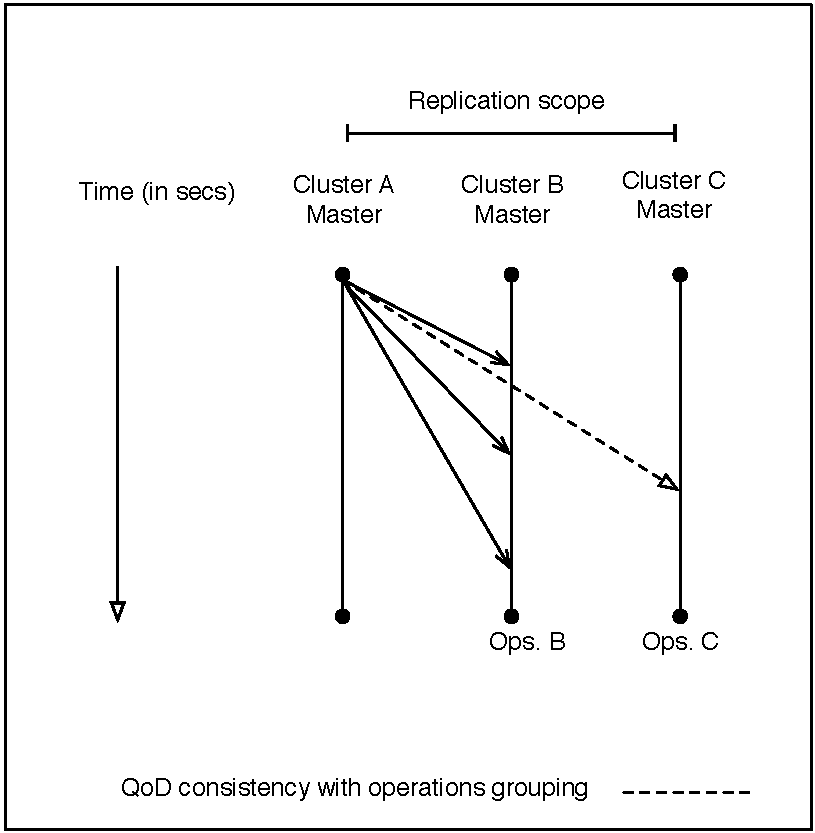
\includegraphics[scale=0.6]{figs/operation-grouping.pdf}
\caption{Resulting scenario of grouping operations in a time-lined based diagram using HBase-QoD versus a regular HBase deployment at Cluster B}
\label{fig-qod-grouping}
\end{figure}

Another experiment that has been conclusive in terms of grouping of operations is the comparison between different QoD levels, in the case of values for vector field K (-, $\sigma$, -). Setting the operation grouping for a small number of updates still shows that a timestamp in the receiving server is the same for every item in the group. The following set of operations is ed in Figures~\ref{fig-shipping-grouping} and ~\ref{fig-receiving-grouping}. The same principle can be applied and has been demonstrated to work in the same fashion for different sets of containers.

%(table_name::columnFamily).

\begin{figure}
\centering
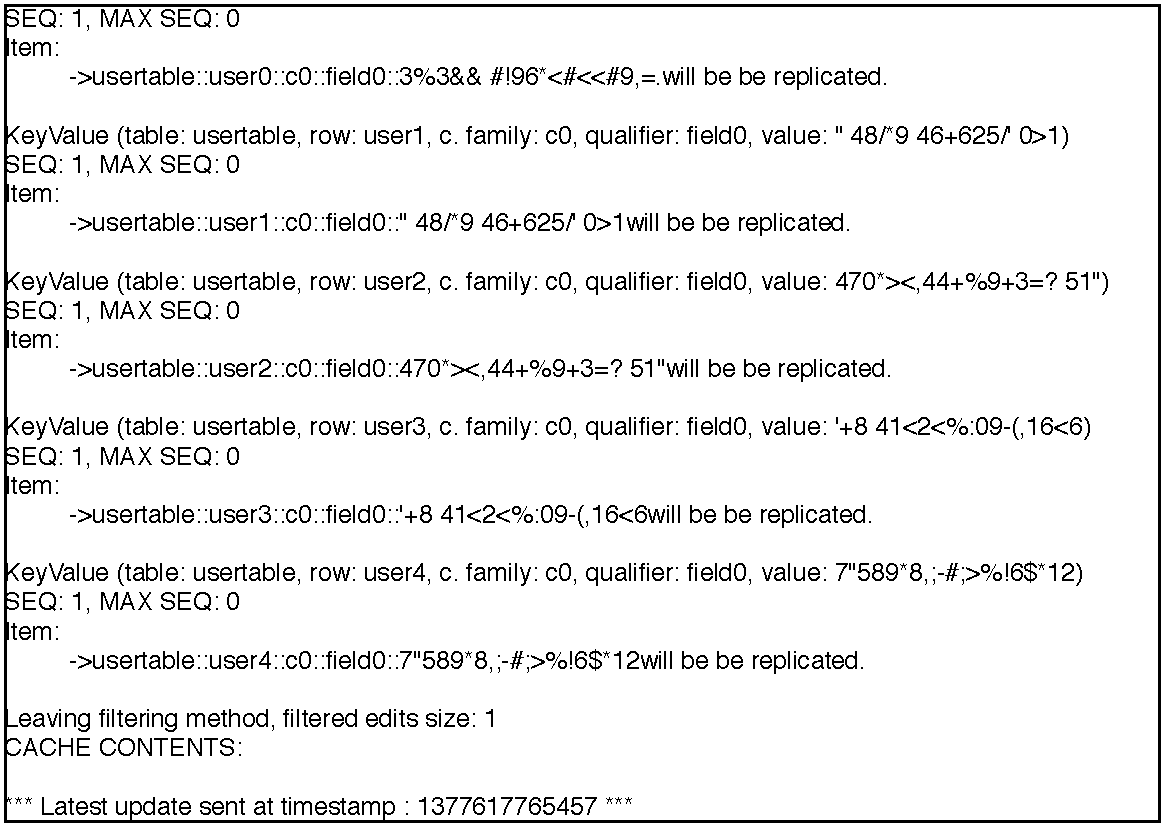
\includegraphics[scale=0.6]{figs/ginja2-grouping-send.pdf}
\caption{Sending from ginja-a2 to ginja-a1}
\label{fig-shipping-grouping}
\end{figure}

In the following Figure~\ref{fig-receiving-grouping}, we observe how the time-stamps for each of the items replicated in a group of operations are the same actually (\textbf{1377617765557}) at the receiving side (Cluster 3 is at server ginja-a1). That is, ensuring they arrive at the same time, once can actually verify the correctness of the solution. Pin-pointing the internal HBase mechanisms we print the time-stamps at the Source and Sink locations by using default built-in reporting mechanisms of the data store. We do not "reinvent the wheel" in that regard. All work is done by leveraging that, and this could be also added to the lists of statistics that is kept into HBase server for tracking the age of updates sent and/or receive. Previously to that, at the sending side, each update is grouped until they are due for replication as a block. Therefore, they only propagate all at once, as showed with the time-stamp below printed for each update~\ref{fig-shipping-grouping}.

\begin{figure}
\centering
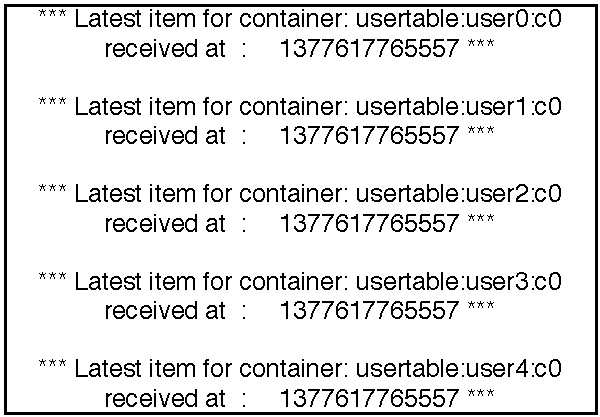
\includegraphics[scale=.6]{figs/ginja1-grouping-receive.pdf}
\caption{Receiving from ginja-a2 in ginja-a1}
\label{fig-receiving-grouping}
\end{figure}
